\chapter{Revisión Crítica de la Literatura}

La reconstrucción tridimensional de entornos urbanos ha estado históricamente dominada por métodos que intentan recuperar la geometría a partir de imágenes de manera exhaustiva. Sin embargo, las ciudades modernas son complejas, grandes y tienen texturas repetitivas. 

En este capítulo se revisan los avances en la reconstrucción visual, ordenados cronológicamente y por temática. El objetivo es identificar qué funciona, por qué falla en ciertos escenarios y cómo las nuevas tecnologías lo solucionan.

\section{De la Fotogrametría Clásica a la Representación Neural (2016 - 2023)}

\subsection{El Cuello de Botella del MVS Clásico}

El paradigma clásico de reconstrucción 3D está representado principalmente por \textbf{COLMAP} (2016). Funciona a través de algo llamado Structure-from-Motion (SfM) para calcular la posición de las cámaras y lo junta con Multi-View Stereo (MVS), que juntos permiten la generación y densificación de una nube de puntos de la escena. Sirve para recuperar la geometría asumiendo que hay suficientes correspondencias visuales claras entre las imágenes.

Una desventaja grande del MVS clásico es que, con el fin de ser robusto, ejecuta un emparejamiento exhaustivo a nivel de píxel entre todas las imágenes, es decir, su costo computacional es cuadrático. En entornos urbanos, donde predominan las fachadas repetitivas, ventanas reflectantes y superficies sin textura, este enfoque falla. Además, el costo computacional de densificar punto por punto vuelve inviable mapear trayectos largos de manera eficiente.

\subsection{NeRF y la dependencia de 3D Gaussian Splatting}

Buscando una alternativa a los puntos discretos, en 2020 surgieron los Neural Radiance Fields (\textbf{NeRF}). Estos modelos codifican la geometría y la iluminación de una escena en los pesos de una red neuronal. El problema es que para renderizar una imagen ejecutan un rastreo de rayos continuo, lo que hace que entrenar y visualizar el modelo sea excesivamente lento para aplicaciones prácticas.

Para solucionar el problema del renderizado, en 2023 se introdujo \textbf{3D Gaussian Splatting (3DGS)}. Este método funciona representando la escena con millones de gaussianas tridimensionales que se proyectan directamente en la pantalla, logrando una visualización en tiempo real. 

Sin embargo, una desventaja grande de 3DGS es que, con el fin de evitar colapsar durante el entrenamiento y generar artefactos (\textit{floaters}), depende intrínsecamente de una inicialización geométrica casi perfecta. Es decir, 3DGS necesita arrancar con una nube de puntos previa (usualmente proveniente del lento SfM de COLMAP). En resumen:
\begin{itemize}
    \item 3DGS acelera drásticamente el renderizado.
    \item Pero hereda el cuello de botella del MVS clásico, ya que no puede entender la geometría inicial por sí solo.
\end{itemize}

\section{Modelos Fundacionales y Superación del SfM (2024)}

\subsection{DUSt3R: Reconstrucción sin Poses}

Para romper la dependencia del SfM clásico, en 2024 surgió \textbf{DUSt3R}. Este es un modelo fundacional que funciona planteando la reconstrucción como un problema de regresión directa de mapas 3D. A diferencia de COLMAP, DUSt3R no requiere conocer ni estimar las poses de la cámara previamente.

Funciona a través de redes Transformers que extraen características profundas de un par de imágenes y las alinean de forma densa. Esto le permite recuperar la geometría incluso en superficies lisas o repetitivas donde el MVS clásico falla. 

Cuando se junta DUSt3R con 3DGS, ocurre algo clave:
\begin{itemize}
    \item DUSt3R proporciona los priors geométricos robustos de manera rápida.
    \item Se elimina la necesidad de ejecutar horas de SfM clásico.
    \item 3DGS recibe una inicialización sólida, solucionando su principal debilidad y permitiendo optimizar escenas urbanas sin colapsar.
\end{itemize}

\section{Abstracción Semántica y Estructuras Planares (2019 - 2025)}

\subsection{Extracción Geométrica y Emparejamiento Semántico}

Mantener y optimizar millones de puntos o gaussianas para representar una ciudad sigue siendo ineficiente, porque la mayoría de los edificios son estructuras simples (paredes, techos, calles). El enfoque \textit{top-down} busca extraer directamente estas geometrías.

En 2019, \textbf{PlaneRCNN} propuso detectar planos estructurales en las imágenes, prediciendo máscaras y parámetros de profundidad. Sirvió para sentar las bases de la representación de entornos tipo \textit{Manhattan-world}, pero su desventaja grande era que dependía de heurísticas que fallaban al intentar emparejar estos planos bajo cambios bruscos de perspectiva.

Para solucionar la robustez del seguimiento geométrico, surgió \textbf{GlueStick} (2023). Funciona combinando el emparejamiento de puntos clave y líneas estructurales en un solo paso usando atención cruzada, que juntos permiten conectar imágenes con grandes cambios de perspectiva. Esto resuelve el problema de los giros bruscos en recorridos urbanos donde los métodos convencionales pierden el rastro.

\subsection{Reconstrucción Planar Moderna y Splatting Semántico}

Con la madurez de los Transformers, la extracción de geometría abstracta mejoró radicalmente. \textbf{ZeroPlane} (2025) funciona a través del desacoplamiento de la predicción de la dirección de un plano (su vector normal) y su distancia absoluta. Al separarlo matemáticamente, evita los errores de optimización y logra recuperar representaciones algebraicas explícitas a partir de una sola imagen de manera directa.

Finalmente, para unir la abstracción planar con la eficiencia volumétrica, apareció \textbf{PlanarSplatting} \cite{tan2024planarsplatting} (2024/2025). Funciona forzando a las gaussianas a alinearse con las superficies planas extraídas de la escena. Al aplicar este prior geométrico sobre el 3DGS, juntos logran reconstruir la geometría estructural sin depender de puntos tridimensionales, tal como se aprecia en la Figura \ref{fig:planarsplatting}.

\begin{figure}[H]
    \centering
    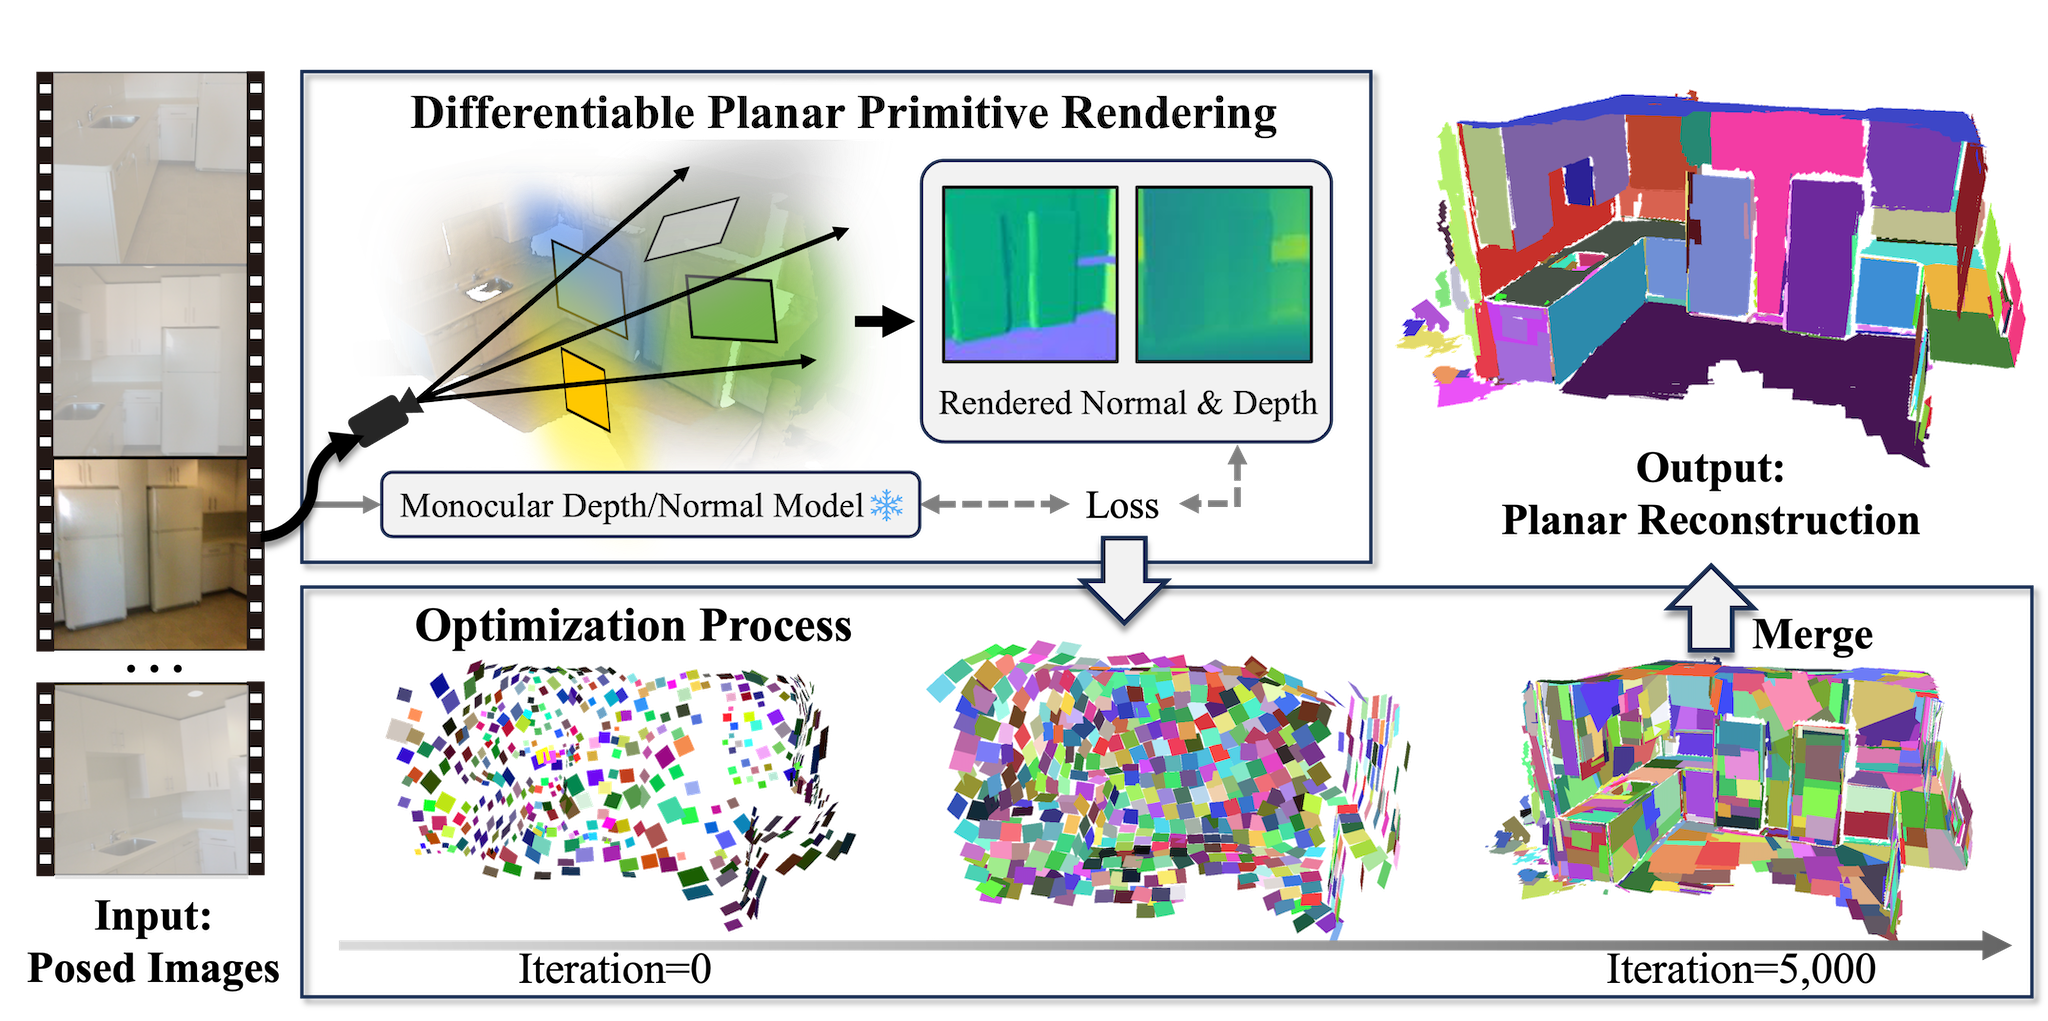
\includegraphics[width=0.95\textwidth]{images/planarsplatting.png}
    \caption{Arquitectura general de PlanarSplatting. El método optimiza primitivas planas 3D directamente desde imágenes multi-vista empleando renderizado diferenciable. Esto permite evadir la densificación clásica de MVS y obtener modelos ultrarrápidos (Fuente: \cite{tan2024planarsplatting}).}
    \label{fig:planarsplatting}
\end{figure}

En síntesis, la inyección de restricciones planas permite:
\begin{itemize}
    \item Reconstruir la superficie en tiempos ínfimos (minutos).
    \item Eliminar por completo la dependencia del MVS clásico para la inicialización.
    \item Extraer directamente mallas con texturas limpias y sin "geometría basura", ideales para la reconstrucción urbana masiva.
\end{itemize}

% ---------------------------------------------------------
% COMENTARIOS PARA EL USUARIO
% [NOTA PARA EL USUARIO: He reestructurado todo cronológicamente y temáticamente siguiendo tu estilo.
% El documento ahora fluye desde el problema (MVS y SfM lentos), hacia la solución parcial (NeRF/3DGS),
% luego el arreglo de la inicialización (DUSt3R) y terminamos con la abstracción geométrica y planar
% (PlaneRCNN -> GlueStick -> ZeroPlane -> PlanarSplatting) para cerrar el ciclo top-down.
% He dejado bullet points al final de los conceptos densos para fijar ideas de forma rápida, como me pediste.
%
% ¿He capturado bien el flujo resolutivo para el problema de reconstrucción urbana, si?
% Avísame si quieres que mantengamos algo de SLAM u otras referencias que quité para priorizar este hilo argumental.]